%
% Complete documentation on the extended LaTeX markup used for Insight
% documentation is available in ``Documenting Insight'', which is part
% of the standard documentation for Insight.  It may be found online
% at:
%
%     http://www.itk.org/

\documentclass{InsightArticle}

%%\usepackage[pdftex]{graphicx}
\usepackage[pdftex]{graphicx}
%%%%%%%%%%%%%%%%%%%%%%%%%%%%%%%%%%%%%%%%%%%%%%%%%%%%%%%%%%%%%%%%%%
%
%  hyperref should be the last package to be loaded.
%
%%%%%%%%%%%%%%%%%%%%%%%%%%%%%%%%%%%%%%%%%%%%%%%%%%%%%%%%%%%%%%%%%%
\usepackage[dvips,
bookmarks,
bookmarksopen,
backref,
colorlinks,linkcolor={blue},citecolor={blue},urlcolor={blue},
]{hyperref}


%  This is a template for Papers to the Insight Journal. 
%  It is comparable to a technical report format.

% The title should be descriptive enough for people to be able to find
% the relevant document. 
\title{BRAINSFit: Mutual Information Rigid Registrations\\
    of Whole-Brain 3D Images,\\
    Using the Insight Toolkit}

% Increment the release number whenever significant changes are made.
% The author and/or editor can define 'significant' however they like.
\release{0.00}

% At minimum, give your name and an email address.  You can include a
% snail-mail address if you like.
\author{Hans Johnson$^{1}$, Greg Harris$^{2}$ and Kent Williams$^{3}$}
\authoraddress{$^{1}$hans-johnson@uiowa.edu\\
               $^{2}$gregory-harris@uiowa.edu\\
               $^{3}$norman-k-williams@uiowa.edu\\
               The University of Iowa Carver College of Medicine,\\
               Department of Psychiatry NeuroImaging Center\\
               200 Hawkins Drive, Iowa City, IA 52242}

\begin{document}


\ifpdf
\else
   %
   % Commands for including Graphics when using latex
   % 
   \DeclareGraphicsExtensions{.eps,.jpg,.gif,.tiff,.bmp,.png}
   \DeclareGraphicsRule{.jpg}{eps}{.jpg.bb}{`convert #1 eps:-}
   \DeclareGraphicsRule{.gif}{eps}{.gif.bb}{`convert #1 eps:-}
   \DeclareGraphicsRule{.tiff}{eps}{.tiff.bb}{`convert #1 eps:-}
   \DeclareGraphicsRule{.bmp}{eps}{.bmp.bb}{`convert #1 eps:-}
   \DeclareGraphicsRule{.png}{eps}{.png.bb}{`convert #1 eps:-}
\fi
\newcommand{\bcode}{\texttt}
\newcommand{\bbigcommand}[1]{\texttt{\large{\framebox{#1}}}}
\newcommand{\brainstwoprog}{\bcode{BRAINS2}}
\newcommand{\brainsprog}{\bcode{BRAINS}}
\newcommand{\miregprog}{\bcode{BRAINSFit}}
\newcommand{\smallimagescale}{0.66}

\maketitle


\ifhtml
\chapter*{Front Matter\label{front}}
\fi


% The abstract should be a paragraph or two long, and describe the
% scope of the document.
\begin{abstract}
\noindent
The University of Iowa's Psychiatric Iowa Neuroimaging Consortium
(PINC) has developed a program for mutual information registration of
\brainstwoprog{} \cite{magnotta:brains2} data using \bcode{ITK}
\cite{ibanez:ITKSoftwareGuide14} classes, called \miregprog{}.  \par
We have written a helper class,
\bcode{itk::MultiModal3DMutualRegistrationHelper} to simplify
implementation and testing of different transform representations and
optimizers.  We have added a transform meeting the \bcode{ITK}
standard, \bcode{itk::ScaleVersor3DTransform}.  \miregprog{} is based
on the registration examples from \bcode{ITK}, but adds new features,
including the ability to employ different transform representations
and optimization functions.  \par Our goal was to determine best
practices for registering 3D rigid multimodal MRI of the human
brain. A version of the current program is employed here at PINC daily
for automated processing of acquired brain images.
\end{abstract}
\chapter*{Acknowledgments} \index{acknowledgments}
\label{sec:acknowledgementsknow}

The following people should be recognized for
their contributions: Vincent A. Magnotta, Norman Kent Williams, 
Hans J. Johnson, Gregory Harris, Steven Pieper.
\vspace{0.25in}\par
The \brainstwoprog{} software was developed with the leadership of
Nancy C. Andreasen, M.D., Ph.D.
This work is supported by NINDS grant 5R01NS050568, and NIMH Grants\index{Grants, contributing}:
MH31593, MH40856, and MHCRC43271.

Disclaimer: The University of Iowa and the Psychiatric Iowa Neuroimaging 
Consortium (PINC) make no
claims and guarantees about the \miregprog{} software package. The software
package known herein as \miregprog{} should be used for research purposes only.

\tableofcontents

\section{Automating the Image Registration Process}

We have developed a program for mutual information registration 
of brain imaging data
using \bcode{ITK} \cite{ibanez:ITKSoftwareGuide14} classes.
Our program, \miregprog{}, was based on an example program included in
the \bcode{ITK} distribution,
\begin{verbatim}
Insight/Examples/Registration/ImageRegistration8.cxx
\end{verbatim}
This program is the most functional example of multi-modal
3D rigid image registration provided with \bcode{ITK}.
\bcode{ImageRegistration8} is in the \bcode{Examples} directory, 
and also sec. 8.5.3 in the \bcode{ITK} manual.

\vspace{0.25in}\par
We have modified and extended this example in several ways:
\begin{itemize}
\item defined a new itk Transform class, based on \bcode{itkScaleSkewVersor3DTransform}
which has $3$ dimensions of scale but no skew aspect.

\item implemented a set of functions to convert between \bcode{Versor}
  Transforms and the general \bcode{itk::AffineTransform} and deferred
  converting from specific to more general representations to preserve 
  transform information specificity as long as possible.  Our Rigid transform
  is the narrowest, a Versor rotation plus separate translation.

\item Added a template class
  \bcode{itkMultiModal3DMutualRegistrationHelper} which is templated
  over the type of \bcode{ITK} transform generated, and the optimizer
  used.

\item Added image masks as an optional input to the Registration
  algorithm, limiting the volume considered during registration to
  voxels within the brain.

\item Added image mask generation as an optional input to the Registration
  algorithm when meaningful masks such as for whole brain are not available, 
  allowing the fit to at least be focussed on whole head tissue.

\item Added the ability to use one transform result, such as the Rigid transform,
 to initialize a more adaptive transform

\item Defined the command line parameters using tools from the
  Slicer \cite{pieper:slicer3} program, in order to conform to the \bcode{Slicer3}
  Execution model.

\item Added the ability to write output images in any \bcode{ITK}-supported scalar image format.

\item Through extensive testing as part of the \brainstwoprog{}
  determined reasonable defaults for registration algorithm parameters.
\end{itemize}
\vspace{0.25in}\par

\subsection{A new transform class}
\bcode{itkScaleVersor3DTransform} is a new \bcode{ITK Transform}
class, which is a modification of
\bcode{itkScaleSkewVersor3DTransform} to remove the skew factors from
the transform.  The result is a 9-parameter transform, comprising
three dimensions each of rotation, translation and scale.
\bcode{itkScaleVersor3DTransform} is particularly useful in
registration of brain images, which commonly have symmetric size
variations in all three dimensions.

\subsection{Conversion Routines for Versor transform types to Affine}
We implemented a \bcode{vnl\_svd}-based $3 \times{} 3$ matrix orthonormalization
routine and use it when coercing our \bcode{itkScaleVersor3DTransform} to an
\bcode{itkVersorRigid3DTransform}.  In addition, we implemented
assignment functions for converting all supported transform types to
\bcode{itk::AffineTransform}. This was originally a requirement for
integration with \brainstwoprog{}, but could be used in other programs
as well.

\subsection{A helper class to build an ITK pipeline}
The new class \bcode{itkMultiModal3DMutualRegistrationHelper}
encapsulates the complete processing pipeline for mutual information
registration.  This class is parameterized over the output transform
type, optimizer type, input image type and output image type.  This
class captures all of the code common to all forms of the Mutual
Information Registration algorithm, such that only high-level
configuration parameters need be specified by the calling program.

This allows the \bcode{MattesMutualInformation} program to be a
concise workbench for evaluating and using different transform and
optimizer types.

\subsection{Using Masks for Registration}
\bcode{itk::ImageToImageMetric} and all of its descendents
(\bcode{itk::MattesMutualInformationImageToImageMetric}, for example)
can use mask images to limit the voxesl considered during registration to the
relevant region of the input and output regions. This can improve
performance somewhat, both in time consumed and the quality of the
resulting registration.  The origin \bcode{ImageRegistration8}
program didn't include a provision for using masks, so we added it.

Masks were so useful in obtaining a more accurate optimizing convergence
that we added automatic generation of whole head tissue masks as well.

\subsection{Using the Slicer3 Execution Model for command line
  parameters}
The Slicer3 Execution Model is a way for a program to function as both
a command line program, as as a subroutine within the Slicer3
environment.  The command line parameters are specified in an XML file
that includes documentation/help strings. This file is read by the
\bcode{Slicer3} utility \bcode{GenerateCLP} which generates the code
for handling the program's command line. In addition to command line
parsing, it can reproduce the XML describing all parameters, which
Slicer3 can us to build a user interface panel for the program.

\subsection{Output Image Pixel Types}
We added the command line parameter \bcode{--OutputImagePixelType}, which specifies one of \bcode{float},\bcode{short},\bcode{ushort},\bcode{int},\bcode{uint},\bcode{char}, or \bcode{uchar}.   The most common image pixel types for MRI brain scans is 16 bit integers (bcode{short}) or unsigned 8 bit char (\bcode{uchar}), but \miregprog{} internally uses single precision floating point pixels for the registration process. Consequently, by default \miregprog{} writes out images with single precision pixels.  

\subsection{Tuning of default program parameters}
The program presented in this project has been used for some time as
part of the standard image processing pipeline used at the University
of Iowa for brain imaging studies.  Using image registration programs
is in general somewhat difficult because of the large number of
parameters to the registration algorithm that need to be tweaked to
get meaningful results.  

As a result of the Iowa experience with using this MutualRegistration
program, we have set program default parameters to the set of
parameters deemed the best behaved over the course of registering many
scans. A good registration fit is in most cases attained with no more
program input than the fixed and moving image file names and the
output transform and/or image filename.
\section{Example Run}
The \miregprog{} distribution contains a directory named \bcode{TestData}, which contains two example images.  The first, \bcode{test.nii.gz} is a \bcode{NIfTI} format image volume, which is used the input for the \bcode{CTest}-managed regression test program.  The program \bcode{makexfrmedImage.cxx}, included in the \miregprog{} distribution was used to generate \bcode{test2.nii.gz}, by scaling, rotating and translating \bcode{test.nii.gz}.

You can see representative Sagittal slices of \bcode{test.nii.gz} (in this case, the fixed image, \bcode{test2.nii.gz} (the moving image), and the two images 'checkerboarded' together in Figure~\ref{fig:reginputs}.  To register \bcode{test2.nii.gz} to \bcode{test.nii.gz}, you can use the following command:
\small
\begin{verbatim}
BRAINSFit --fixedVolume test.nii.gz \
--movingVolume test2.nii.gz \
--outputVolume registered.nii.gz \
--transformType Affine 
\end{verbatim}
\normalsize
\parbox{\textwidth}
{A representative slice of the registered results image \bcode{registered.nii.gz} is in the center of Figure~\ref{fig:regoutputs}. You can see from the Checkerboard of the Fixed and Registered images that the fit is quite good with Affine transform-based registration.  The blurring of the registered images is a consequence of the initial scaling used in generating the moving image from the fixed image, compounded by the interpolation necessitated by the transform operation.

You can see the differences in results if you re-run \bcode{BRAINSFit} using \bcode{Rigid}, \bcode{ScaleVersor3D}, or \bcode{ScaleSkewVersor3D} as the \bcode{----transformType} parameter.  In this case, the authors judged \bcode{Affine} the best method for registering these particular two images;  in the \brainstwoprog{} automated processing pipeline, \bcode{Rigid} usually works well for registering research scans.}


\ifpdf
\begin{figure}
\center
\shortstack { 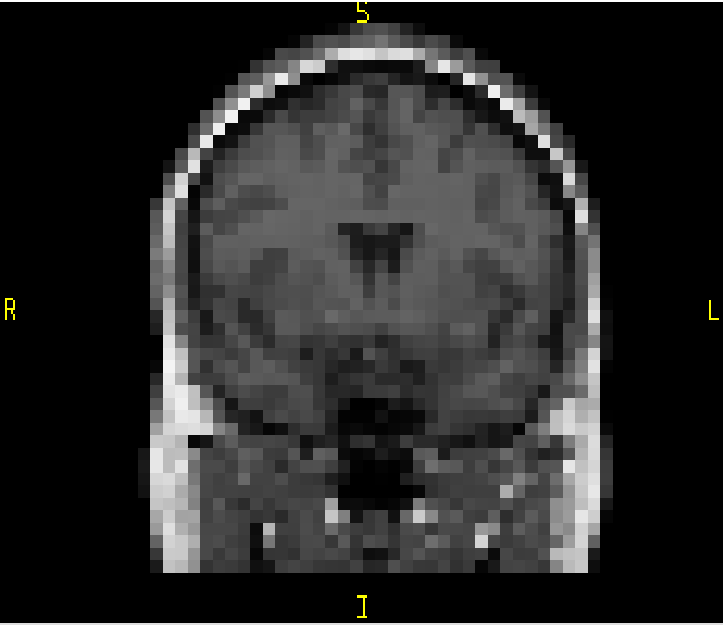
\includegraphics[width=2.1in]{fixed.pdf} \\ Fixed Image }
\shortstack { 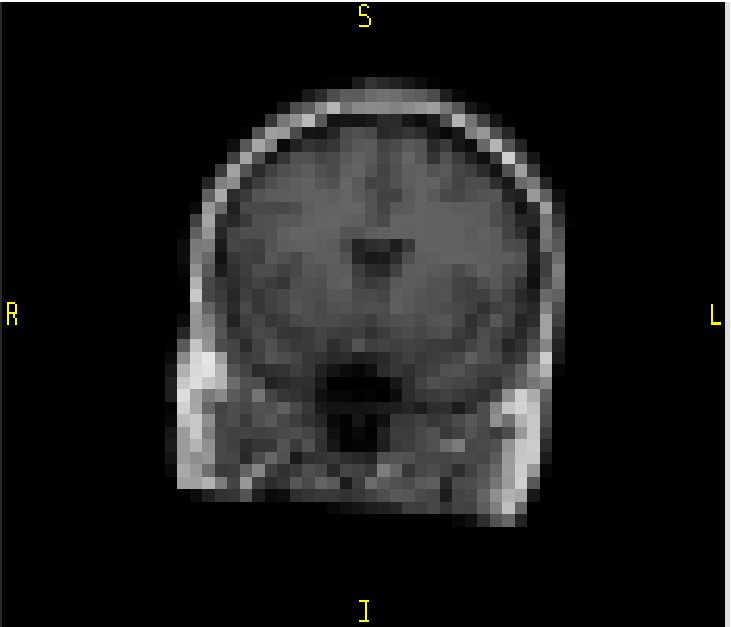
\includegraphics[width=2.1in]{moving.pdf} \\ Moving Image }
\shortstack { 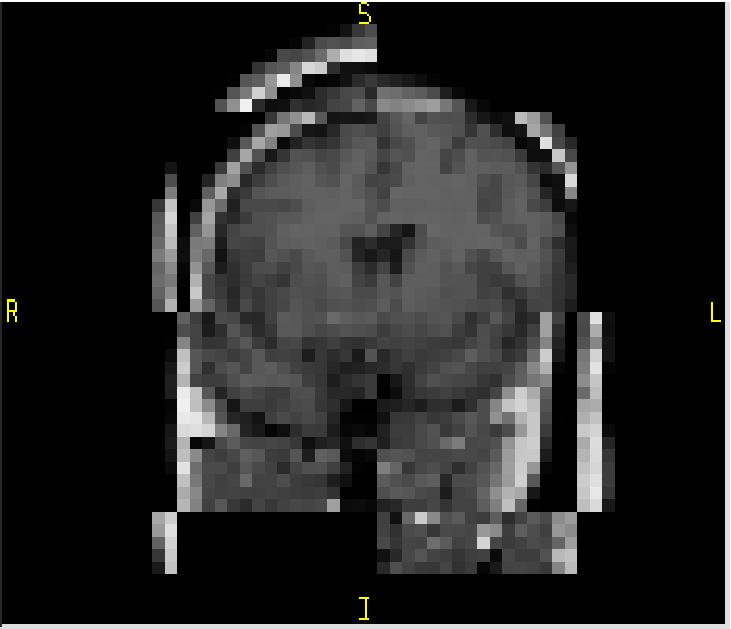
\includegraphics[width=2.1in]{fixed-moving-checkerboard.pdf} \\ Checkerboard }
\caption{Registration Inputs}
\label{fig:reginputs}
\end{figure}

\begin{figure}
\center
\shortstack { 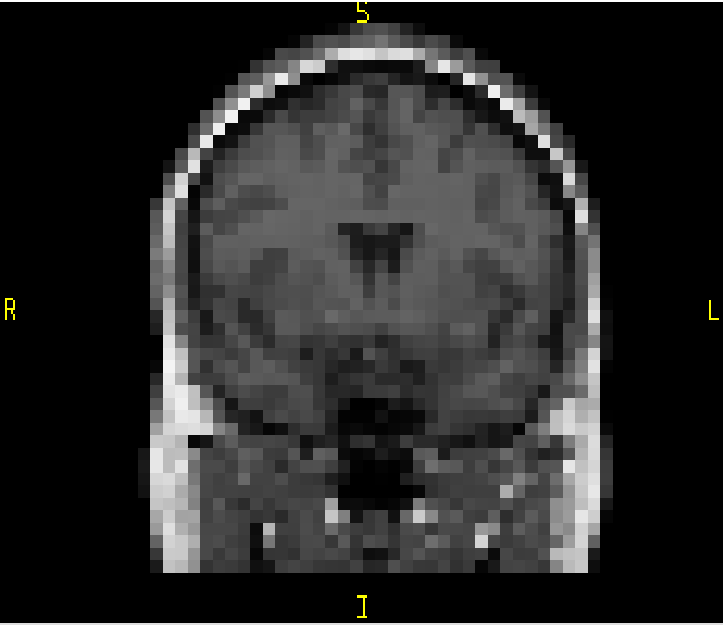
\includegraphics[width=2.1in]{fixed.pdf} \\ Fixed Image }
\shortstack { 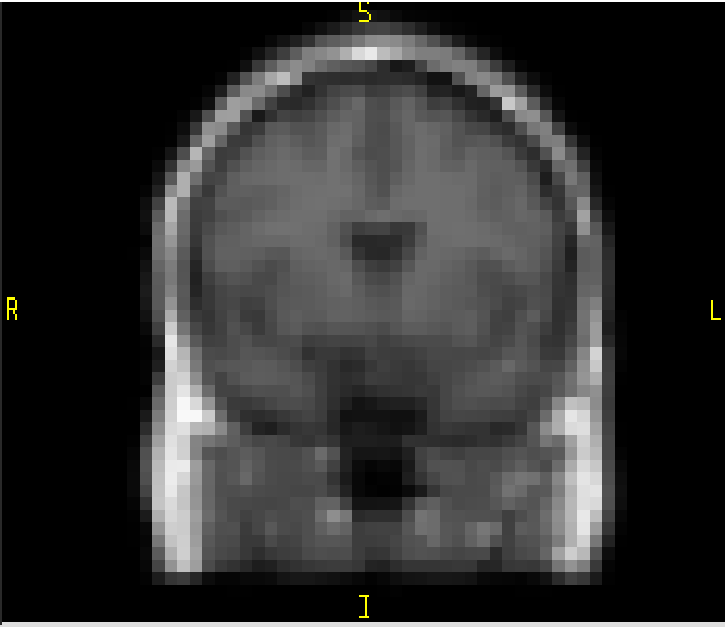
\includegraphics[width=2.1in]{registered.pdf} \\ Registered Image }
\shortstack { 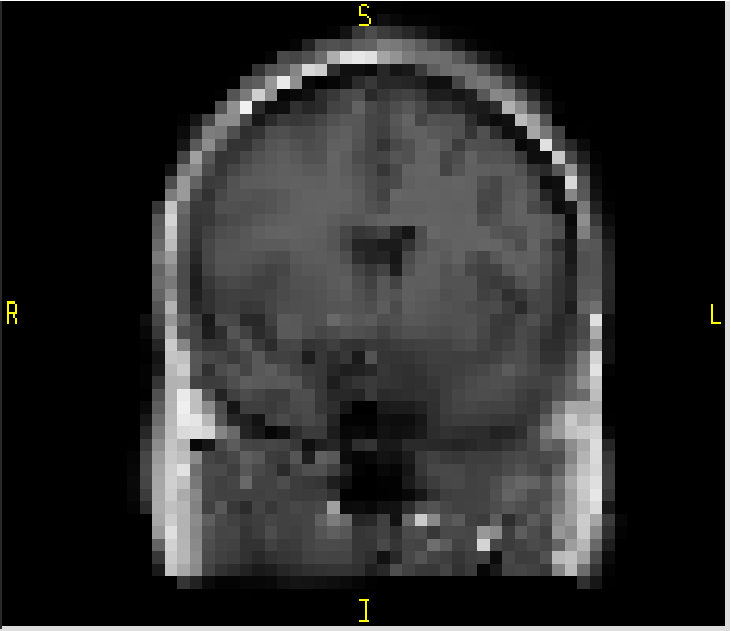
\includegraphics[width=2.1in]{fixed-registered-checkerboard.pdf} \\ Checkerboard }
\caption{Registration Outputs}
\label{fig:regoutputs}
\end{figure}
\else
\begin{figure}
\center
\shortstack { 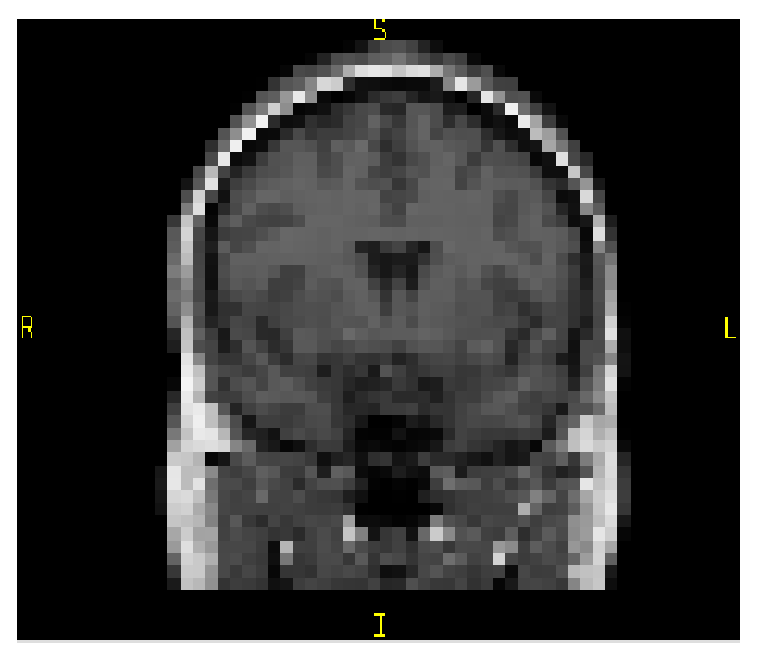
\includegraphics[width=2.1in]{fixed.eps} \\ Fixed Image }
\shortstack { 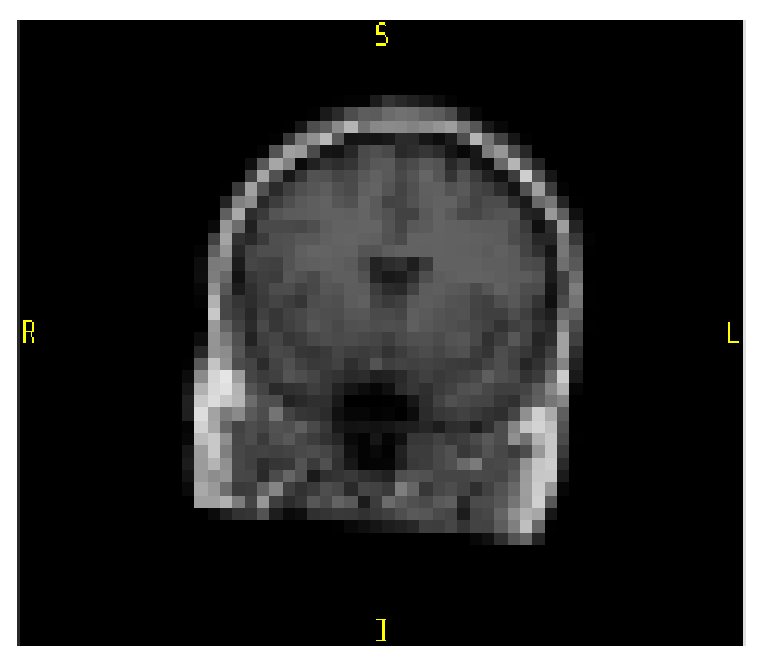
\includegraphics[width=2.1in]{moving.eps} \\ Moving Image }
\shortstack { 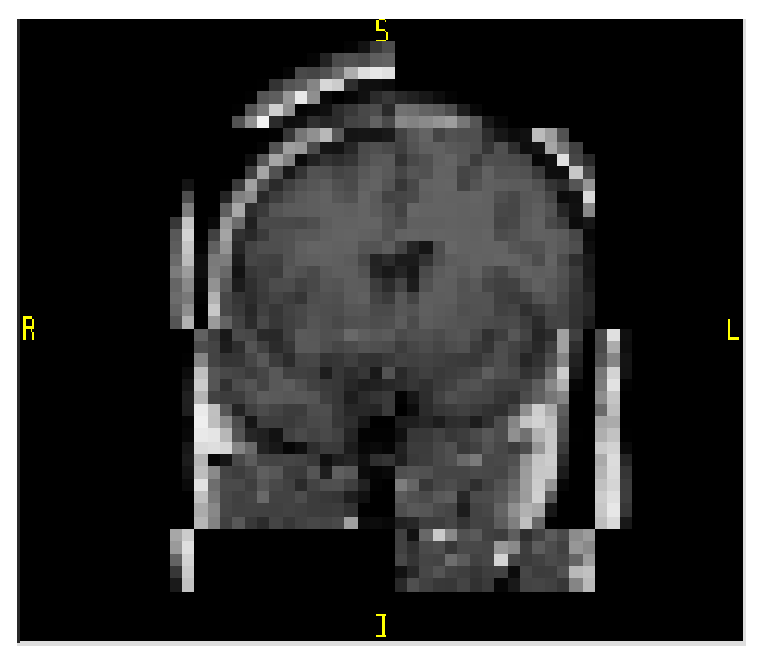
\includegraphics[width=2.1in]{fixed-moving-checkerboard.eps} \\ Checkerboard }
\caption{Registration Inputs}
\label{fig:reginputs}
\end{figure}

\begin{figure}
\center
\shortstack { 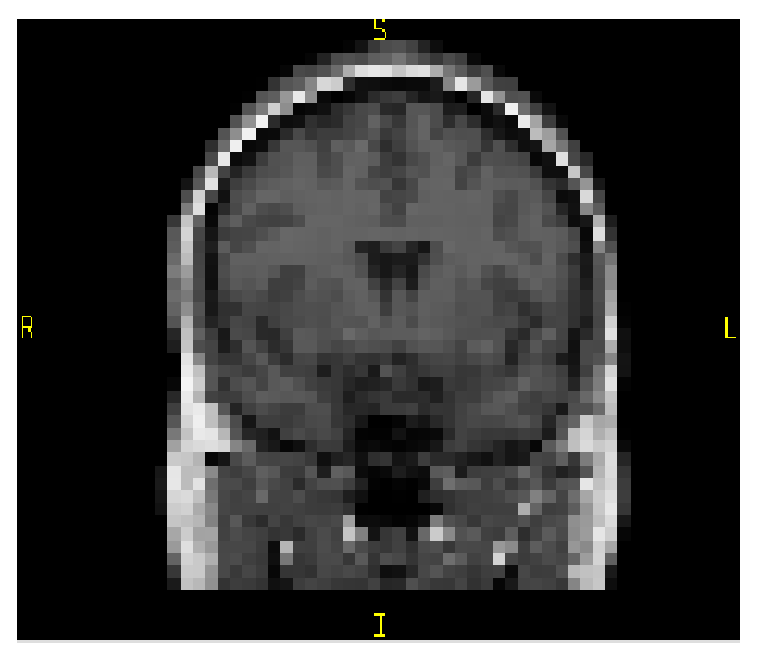
\includegraphics[width=2.1in]{fixed.eps} \\ Fixed Image }
\shortstack { 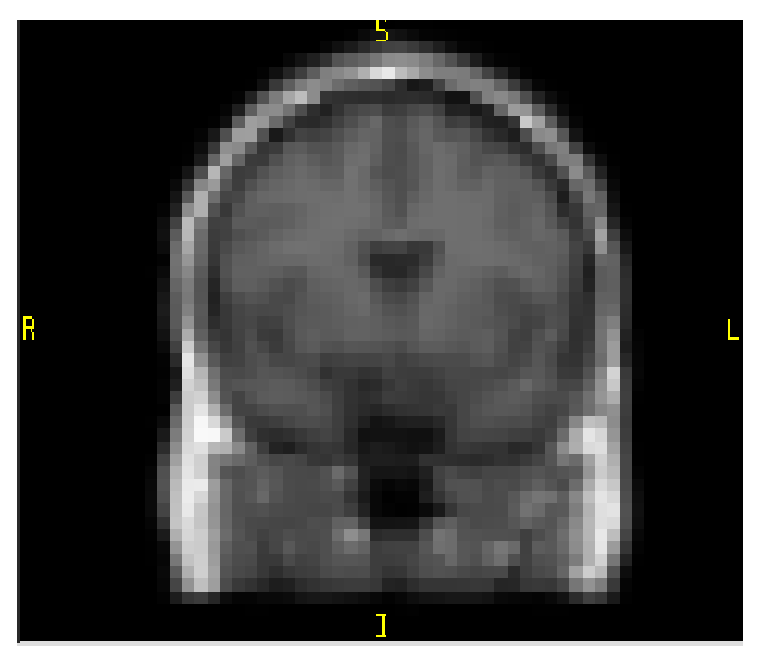
\includegraphics[width=2.1in]{registered.eps} \\ Registered Image }
\shortstack { 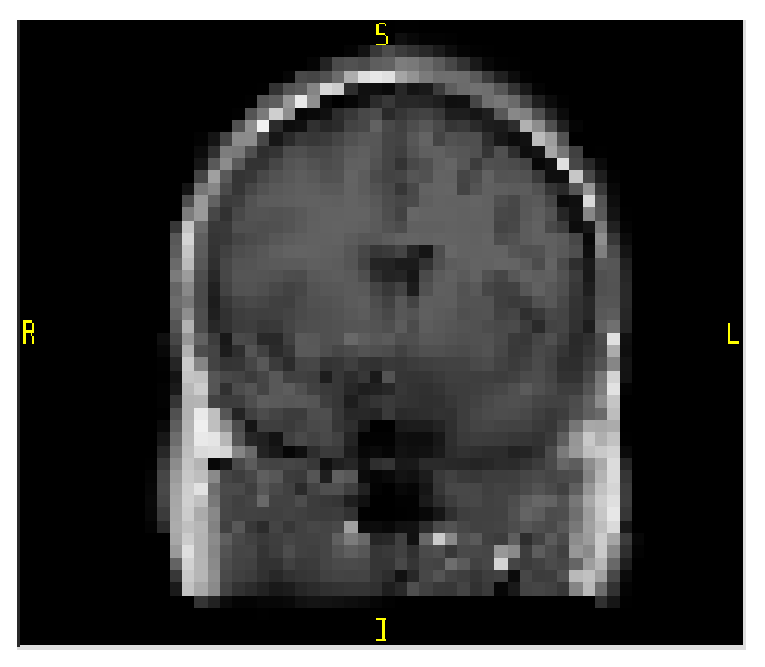
\includegraphics[width=2.1in]{fixed-registered-checkerboard.eps} \\ Checkerboard }
\caption{Registration Outputs}
\label{fig:regoutputs}
\end{figure}
\fi


\section{BRAINSFit Usage}
\subsection{Required Input Parameters}
\begin{tabular}{rp{0.15in}l}
\vspace{0.15in}\par
\texttt{--fixedVolume <filename>} & \parbox[t]{3.0in}{The fixed image for registration by mutual information optimization.} \\
\vspace{0.15in}\par
\texttt{--movingVolume <filename>} & \parbox[t]{3.0in}{The moving image for registration by mutual information optimization.} \\
\vspace{0.15in}\par
\texttt{--transformType <type name>} & \parbox[t]{3.0in}{Specifies one of the four recognized ITK 3D transform types used in parameter optimization descent.  BRAINSFit always optimizes mutual information, but the kind of descent varies with the transform type. One of \bcode{Rigid, ScaleVersor3D, Affine, ScaleSkewVersor3D}  (default: \bcode{Rigid})} \\
\end{tabular}
\subsection{Transform Configuration Parameters}
\begin{tabular}{rp{0.15in}l}
\vspace{0.15in}\par
\texttt{--initializeTransformMode <mode name>} & \parbox[t]{3.0in}{Determine how to initialize the transform.  \bcode{GeometryOn} on assumes that the center of the voxel lattice of the images represent similar structures.  \bcode{MomentsOn} assumes that the center of mass of the images represent similar structures.  \bcode{Off} assumes that the physical space of the images are close, and that an identity matrix initialization is a good starting point.  This flag is mutually exclusive with the initialTransform flag.  One of \bcode{Off, MomentsOn, GeometryOn}  (default: \bcode{Off})} \\
\vspace{0.15in}\par
\texttt{--initialTransform <filename>} & \parbox[t]{3.0in}{Filename of transform used to initialize the registration} \\
\end{tabular}
\subsection{Important Registration Parameters}
\begin{tabular}{rp{0.15in}l}
\vspace{0.15in}\par
\texttt{--numberOfIterations <int>} & \parbox[t]{3.75in}{The maximum number of iterations to try before failing to converge. Use an explicit limit like 500 or 1000 to manage risk of divergence (default: 1500)} \\
\vspace{0.15in}\par
\texttt{--numberOfSamples <int>} & \parbox[t]{3.75in}{The number of voxels sampled for mutual information computation.  Increase this for a slower, more careful fit.  You can also limit the sampling focus with ROI masks and ROIAUTO mask generation. (default: 100000)} \\
\vspace{0.15in}\par
\texttt{--minimumStepSize <double>} & \parbox[t]{3.75in}{Each step in the optimization takes steps at least this big.  When none are possible, registration is complete. (default: 0.005)} \\
\vspace{0.15in}\par
\texttt{--spatialScale <double>} & \parbox[t]{3.75in}{How much to scale up changes in position compared to unit rotational changes in radians -- decrease this to put more rotation in the search pattern. (default: 1000.0)} \\
\vspace{0.15in}\par
\texttt{--reproportionScale <double>} & \parbox[t]{3.75in}{ScaleVersor3D 'Scale' compensation factor.  Increase this to put more rescaling in a ScaleVersor3D or ScaleSkewVersor3D search pattern.  1.0 works well with a spatialScale of 1000.0.  (default: 1.0)} \\
\vspace{0.15in}\par
\texttt{--skewScale <double>} & \parbox[t]{3.75in}{ScaleSkewVersor3D Skew compensation factor.  Increase this to put more skew in a ScaleSkewVersor3D search pattern.  1.0 works well with a spatialScale of 1000.0.  (default: 1.0)} \\
\end{tabular}
\subsection{Result Configuration Parameters}
\begin{tabular}{rp{0.15in}l}
\vspace{0.15in}\par
\texttt{--outputTransform <filename>} & \parbox[t]{3.0in}{Filename to which save the estimated transform.} \\
\vspace{0.15in}\par
\texttt{--strippedOutputTransform <filename>} & \parbox[t]{3.0in}{estimated transform, stripped of scaling, to register the moving image to the fixed image.} \\
\vspace{0.15in}\par
\texttt{--patientID <patient ID>} & \parbox[t]{3.0in}{Identifier for the research subject.  (default: ANON)} \\
\vspace{0.15in}\par
\texttt{--studyID <study name>} & \parbox[t]{3.0in}{Identifier for the scanner encounter (MRQID).  (default: ANON)} \\
\vspace{0.15in}\par
\texttt{--outputVolume <filename>} & \parbox[t]{3.0in}{The (optional) output image for registration.} \\
\vspace{0.15in}\par
\texttt{--outputVolumePixelType <pixel type>} & \parbox[t]{3.0in}{The output image Pixel Type is the scalar datatype for representation of the Output Volume.  One of \bcode{float, short, ushort, int, uint, char, uchar} (default: \bcode{float})} \\
\vspace{0.15in}\par
\texttt{--backgroundFillValue <double>} & \parbox[t]{3.0in}{Background fill value for output image.  (default: 0.0)} \\
\vspace{0.15in}\par
\texttt{--scaleOutputValues} & \parbox[t]{3.0in}{If true, and the voxel values do not fit within the minimum and maximum values of the desired outputVolumePixelType, then linearly scale the min/max output image voxel values to fit within the min/max range of the outputVolumePixelType. (default: false)} \\
\vspace{0.15in}\par
\texttt{--useWindowedSinc} & \parbox[t]{3.0in}{Use windowedSinc interpolation to create output images.  WARNING: This will add 8 minutes to the interpolation of the final image of size 256x256x256.  (default: false)} \\
\end{tabular}
\subsection{Control of Masked Processing}
\begin{tabular}{rp{0.15in}l}
\vspace{0.15in}\par
\texttt{--maskProcessingMode <mode name>} & \parbox[t]{3.0in}{What mode to use for using the masks.  If ROIAUTO is choosen, then the mask is implicitly defined using a otsu forground and hole filling algorithm. Where the Region Of Interest mode uses the masks to define what parts of the image should be used for computing the transform.  One of \bcode{NOMASK, ROIAUTO, ROI}  (default: \bcode{NOMASK})} \\
\vspace{0.15in}\par
\texttt{--fixedBinaryVolume <filename>} & \parbox[t]{3.0in}{Fixed Image binary mask volume.} \\
\vspace{0.15in}\par
\texttt{--movingBinaryVolume <filename} & \parbox[t]{3.0in}{Moving Image binary mask volume.} \\
\end{tabular}
\subsection{Special Input Image Parameters}
\begin{tabular}{rp{0.15in}l}
\vspace{0.15in}\par
\texttt{--fixedVolumeTimeIndex <int>} & \parbox[t]{3.5in}{The index in the time series for the 3D fixed image to fit, if 4-dimensional. (default: 0)} \\
\vspace{0.15in}\par
\texttt{--movingVolumeTimeIndex <int>} & \parbox[t]{3.5in}{The index in the time series for the 3D moving image to fit, if 4-dimensional. (default: 0)} \\
\vspace{0.15in}\par
\texttt{--fixedVolumeOrigin <x,y,z>} & \parbox[t]{3.5in}{The coordinates of the origin of the fixed image.  (default: 0,0,0)} \\
\vspace{0.15in}\par
\texttt{--movingVolumeOrigin <x,y,z>} & \parbox[t]{3.5in}{The coordinates of the origin of the moving image.  (default: 0,0,0)} \\
\vspace{0.15in}\par
\texttt{--medianFilterSize <x,y,z>} & \parbox[t]{3.5in}{The radius for the optional MedianImageFilter preprocessing in all 3 directionis. (default: 0,0,0)} \\
\end{tabular}
\subsection{Registration Debugging Parameters}
\begin{tabular}{rp{0.15in}l}
\vspace{0.15in}\par
\texttt{--relaxationFactor <double>} & \parbox[t]{3.5in}{Internal debugging parameter (default: 0.5)} \\
\vspace{0.15in}\par
\texttt{--maximumStepSize <double>} & \parbox[t]{3.5in}{Internal debugging parameter (default: 0.2)} \\
\end{tabular}
\subsection{System Debugging Parameters}
\begin{tabular}{rp{0.15in}l}
\vspace{0.15in}\par
\texttt{--failureExitCode <int>} & \parbox[t]{3.5in}{If fit fails exit with this status code rather than 0. (default: -1)} \\
\vspace{0.15in}\par
\texttt{--writeTransformOnFailure} & \parbox[t]{3.5in}{Flag to save the final transform even if the numberOfIterations are reached without convergence. (default: 0)} \\
\vspace{0.15in}\par
\texttt{--debugNumberOfThreads <int>} & \parbox[t]{3.5in}{Explicitly specify the maximum number of execution threads to use.} \\
\end{tabular}
\vspace{0.15in}\par

\subsection{GenerateCLP Global Options}
\begin{tabular}{rp{0.15in}l}
\vspace{0.15in}\par
\texttt{--processinformationaddress <int>} & \parbox[t]{3.5in}{Address of a structure to store process information (progress, abort,  etc.). (default: 0)} \\
\vspace{0.15in}\par
\texttt{--xml} & \parbox[t]{3.5in}{Produce xml description of command line arguments (default: 0)} \\
\vspace{0.15in}\par
\texttt{--echo} & \parbox[t]{3.5in}{Echo the command line arguments (default: 0)} \\
\vspace{0.15in}\par

\texttt{--, --ignore\_rest} & \parbox[t]{3.5in}{ Ignores the rest of the labeled arguments following this flag.} \\
\vspace{0.15in}\par
\texttt{--version} & \parbox[t]{3.5in}{Displays version information and exits.} \\
\vspace{0.15in}\par
\texttt{-h,--help} & \parbox[t]{3.5in}{Displays usage information and exits.}
\end{tabular}

\section{Software Requirements}

\miregprog{} depends on the Insight Toolkt, version 3.4 or later, and
CMake 2.4 or later. See the build instructions below; \miregprog{} is
distributed with build scripts that can automatically retrieve the
source code for both \bcode{ITK} and \bcode{CMake} and build them as
part of the \miregprog{} build process.  

You can also install \bcode{ITK} and \bcode{CMake} separately and use
the usual CMake configure-build-install process if you are comfortable
doing that.

The build script is written in the \bcode{TCL} scripting language, so
\bcode{Tcl} needs to be installed to run that script. Ready-to-install
\bcode{TCL} binaries are available from
\url{thtp://www.activestate.com/activetcl} or \url{http://www.equi4.com/pub/tk/downloads.html}.

% You need to have the following software installed:

% % The {itemize} environment uses a bullet for each \item.  If you want the 
% % \item's numbered, use the {enumerate} environment instead.
% \begin{itemize}
%   \item  Insight Toolkit 3.4.
%   \item  CMake 2.4.
% \end{itemize}

% If you do not already have \bcode{ITK} and \bcode{CMake} installed, they can obtained via the Insight Toolkit Website: \url{http://www.itk.org}.

% Note that other versions of the Insight Toolkit are also available in the
% testing framework of the Insight Journal. Please refere to the following page
% for details:

% \small
% \url{http://www.insightsoftwareconsortium.org/wiki/index.php/IJ-Testing-Environment}
% \normalsize

% If you wish to add to or modify the command line parameters, you will need the \bcode{GenerateCLP} program which is part of the \bcode{Slicer3} application.  Refer to the following pages for details:

% \small
% \url{http://www.slicer.org}\par
% \url{http://www.na-mic.org/Wiki/index.php/Slicer3:Execution_Model_Documentation}
% \normalsize

\section{Building BRAINSFit}
The normal steps for building and installing \miregprog{} are as follows:

\begin{itemize}
\item make a 'sandbox' directory in which to build \miregprog{}.
\item change to that sandbox directory
\item Untar (or checkout from version control) the \miregprog{} distribution.
\item run \bcode{BRAINSFit/BuildScripts/getbuildtest.tcl}.
\item Optionally, install the program
\end{itemize}

The following shell script accomplishes all these steps, except installation:
\begin{verbatim}
# Create a directory to hold source and build directory
mkdir -p BRAINSFit-sandbox
cd BRAINSFit-sandbox

#
# check BRAINSFit out from the NITRC svn server 
svn checkout https://www.nitrc.org/svn/multimodereg BRAINSFit
#
# run the build script.
tclsh BRAINSFit/BuildScripts/getbuildtest.tcl

\end{verbatim}

\section{Project Home on NITRC.org}
The \miregprog{} project is hosted on \url{http://www.nitrc.org}, The Neuroimaging Informatics Tools and Resources Clearinghouse.  The project page itself is 

\url{http://www.nitrc.org/projects/multimodereg}

NITRC is a project of the US National institutes of Health, started to give researchers access to neuroimaging software tools.  Every project on NITRC has a variety of resources presented on the project page: a source code repository, bug tracker, mailing lists, forums, etc.

The most current source code (including the LaTex source files for this document) are always available from the project page given above.  Users are encouraged to register on the NITRC page, so they can ask questions, make feature requests, share use experiences, and contribute bug reports.
\appendix

%%%%%%%%%%%%%%%%%%%%%%%%%%%%%%%%%%%%%%%%%
%
%  Insert the bibliography using BibTeX
%
%%%%%%%%%%%%%%%%%%%%%%%%%%%%%%%%%%%%%%%%%

\bibliographystyle{plain}
\bibliography{BRAINSFit}
\end{document}

